\documentclass[tikz, border=3mm]{standalone}
\usepackage{tikz}
\usetikzlibrary{arrows.meta, positioning} % For arrow tips and relative positioning

\begin{document}
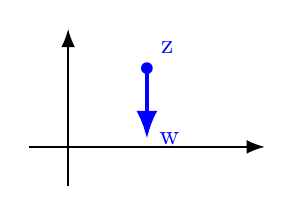
\begin{tikzpicture}[
    >=Latex, % Set default arrow tip style
    dot/.style={fill=blue, circle, inner sep=1.5pt} % Style for the point z
]

    % Axes
    \draw[->, thick] (-0.5, 0) -- (2.5, 0); % x-axis
    \draw[->, thick] (0, -0.5) -- (0, 1.5); % y-axis

    % Define vector points
    \coordinate (z) at (1, 1);      % Start point
    \coordinate (w) at (1, 0.1);    % End point (near x-axis)

    % Draw Point Indicator and Label for z
    \node[dot, label={[blue]above right=1pt:z}] at (z) {}; % Draw dot and label z

    % Draw Vector (make it quite thick)
    \draw[->, blue, ultra thick] (z) -- (w);

    % Label w
    \node[blue, right=1pt of w] {w}; % Position label near end

\end{tikzpicture}
\end{document}